\documentclass{beamer}
%\usepackage[utf8]{inputenc}
\usepackage[T1]{fontenc}
\usepackage[english,brazilian]{babel}
\usetheme{Luebeck}
\usepackage{graphicx}
\usepackage{hologo}
\usepackage{outlines}
\usepackage{listings}
%\usepackage{verbatim}
%\usecolortheme{beaver}
\mode<presentation>
\setbeamertemplate{page number in head/foot}[totalpagenumber]
\AtBeginSection[]
{
  \begin{frame}
    \frametitle{Onde Estamos?}
    \tableofcontents[currentsection]
  \end{frame}
}



\title{O Mundo do \LaTeX}
\subtitle{Seminário \LaTeX - Parte II}


\author{Geraldo Xexéo\inst{1,2}}

\institute[DCC/PESC]{\inst{1}Departamento de Ciências da Computação 
\and
\inst{2}Programa de Engenharia de Sistemas e Computação}

\date[LUDES/LINE]{3o Seminário LUDES/LINE, Março 2020}



\begin{document}


\begin{frame}
\titlepage
\end{frame}

\begin{frame}
\frametitle{Agenda}
\tableofcontents
\end{frame}

\section{Quem inventou}



\subsection{Invenção do \TeX}
\begin{frame}
\frametitle{Invenção do \TeX}

\begin{itemize}
    \item The Art of Computer Programming Vol. I  foi impresso por um método tradicional com fontes móveis
    \item The Art of Computer Programming Vol. II  foi impresso por um método moderno, com fontes eletrônicas
    \item Donald Knuth não gostou do resultado
    \item Inventou e implementou
    \begin{itemize}
        \item \hologo{METAFONT}
        \item \TeX
        \item Literate Programming
    \end{itemize}
\end{itemize}
\end{frame}

\subsection{Invenção do \LaTeX}
\begin{frame}{Invenção do \LaTeX}

\begin{itemize}
    \item Criado em 1983 por Leslie Lamport (SRI)
    \item Macros \TeX~  para uso próprio 
    \item Divulgou de forma mais organizada em 84 e 85
    \item Em 1989 foi formado o time \hologo{LaTeX3}, que lançou o \hologo{LaTeX2e} em 1994
    \item \hologo{LaTeX3} continua em desenvolvimento
\end{itemize}
\end{frame}

\section{Situação Atual}

\subsection{Implementações}
\begin{frame}{Implementações}
\begin{itemize}
    \item Várias implementações de \TeX
    \begin{itemize}
        \item \hologo{pdfTeX} – processador que ficou sendo o mais usado
        \item \hologo{XeTeX} – Unicode + novas fontes
        \item \hologo{LuaTeX} – evolução do pdfTeX onde todos as chamadas internas podem ser acessadas por Lua 
    \end{itemize}
    \item Programs relacionados
    \begin{itemize}
        \item \hologo{BibTeX} – programa original de tratamento de citações e bibliografia
        \item \hologo{biber} – programas recomendados, para usar o bib\LaTeX.
        
    \end{itemize}
\end{itemize}
\end{frame}

\subsection{Tudo sobre \TeX{} e \LaTeX}
\begin{frame}{Tudo sobre \TeX{} e \LaTeX}
    \begin{itemize}
        \item CTAN Comprehensive TEX Archive Network: https://ctan.org/
        \item \TeX Stack Exchange :  https://tex.stackexchange.com/
        \item \TeX FAQ https://texfaq.org/
        \item \TeX User Group – TUG: https://www.tug.org/
        \item The \LaTeX Project: https://www.latex-project.org/
    \end{itemize}
\end{frame}


\section{Como Funciona}
\subsection{Como Funciona}
\begin{frame}{Como Funciona}
\begin{outline}%[enumerate]
  \1 É um compilador que gera um pdf
   \2 Costuma gerar um .dvi
   \1 Nas IDEs, como Overleaf e \TeX Studio, você pode ver o código e o resultado lado a lado
   \1 Previews quase perfeitos já existem
\end{outline}
\end{frame}

\subsection{\TeX  Studio}
\begin{frame}{\TeX  Studio}
\begin{center}
    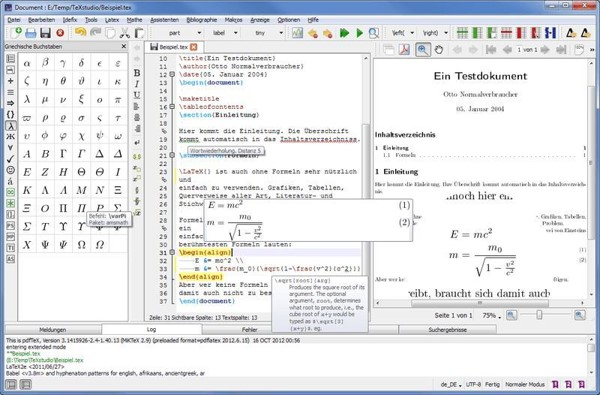
\includegraphics[width=0.8\linewidth]{Images/Picture1.jpg}
\end{center}
\end{frame} 

   
\subsection{Overleaf}
\begin{frame}{Entrada no Overleaf}
\begin{center}
    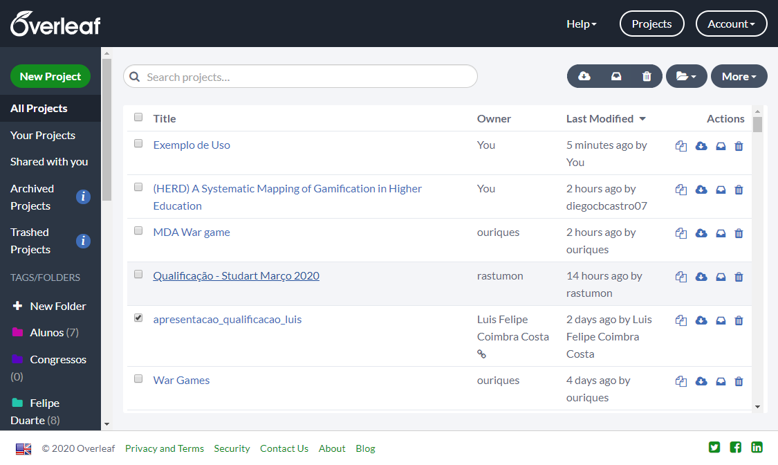
\includegraphics[width=\linewidth]{Images/Picture2.png}
\end{center}    
\end{frame}

\begin{frame}{Edição no Overleaft}
\begin{center}
    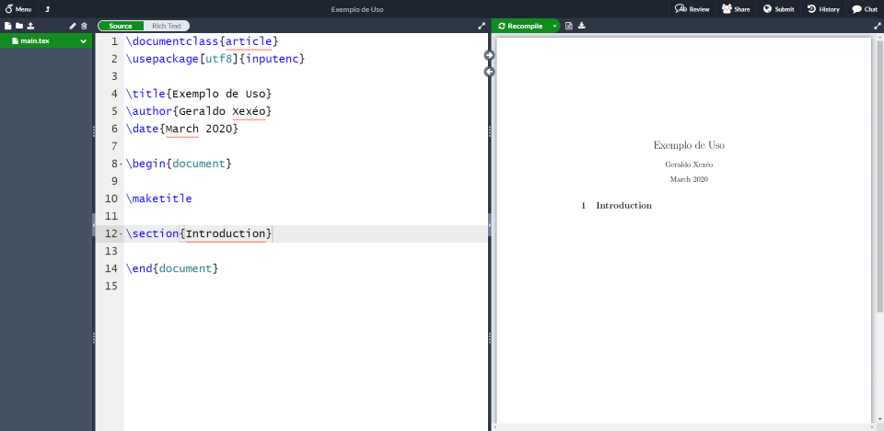
\includegraphics[width=0.8\linewidth]{Images/Picture3.png}
\end{center}    
\end{frame}

\begin{frame}{Menu no Overleaft}
\begin{center}
    \centering
    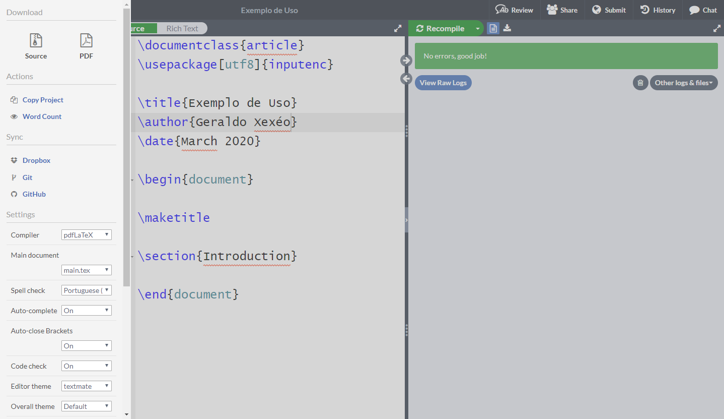
\includegraphics[width=\linewidth]{Images/Picture4.png}
\end{center}    
\end{frame}

\section{Escrevendo em \LaTeX }
\subsection{Documento Mínimo}
\begin{frame}[fragile]{Documento mínimo}
    \begin{block}{\LaTeX}
        \begin{verbatim}
        \documentclass{article}
        \begin{document}
        \end{document}
        \end{verbatim}
    \end{block}
\end{frame}

\subsection{Recomendações}
\begin{frame}{Recomendações I}
    \begin{outline}
        \1 Usar Overleaf enquanto puder
        \1 No PC
            \2 \hologo{MiKTeX} 
            \2 pro\TeX t
            \2 \TeX Live
        \1 No Linux
            \2 Pacote da distribuição
            \2 \TeX Live  –  mais recomendado, por ser atualizado
        \1 No Mac
            \2 Mac\TeX
    \end{outline}
\end{frame}

\begin{frame}{Recomendações II}
    \begin{outline}
    \1 Use o \TeX\ Studio
    \1 Para processar, use o \hologo{LuaTeX} e \hologo{LuaLaTeX}
    \1 Para bibliografia, use o Bib\LaTeX\ (forma do \hologo{biber} 
        \2 Cuidado com estilos que exigem o \hologo{BibTeX}
        \2 Há diferenças sutis de comportamento
    \1 Sempre mantenha seu projeto \LaTeX{}  no Git
        \2 GitHub, GitLab e etc.
    \1 Se vai usar linha de código, construa um makefile ou equivalente
    \end{outline}
\end{frame}

\subsection{Aviso}
\begin{frame}{Aviso}
    \begin{outline}
        \1 O processo ``normal'' inclui compilar 3 ou 4 vezes
        \1 \LaTeX
            \2 Escreve informações necessárias no arquivo .aux
        \1 \hologo{BibTeX} ou \hologo{biber} 
            \2 O \hologo{biber} precisa de 1 passo a menos
        \1 \LaTeX  
            \2 Inclui o .bbl na posição correta
        \1 \LaTeX  
            \2 Processa todos os rótulos corretamente
    \end{outline}
\end{frame}

\begin{frame}
\Huge \center
Obrigado!
\end{frame} 

\begin{frame}{Contato}
\begin{center}
    
\includegraphics[width=\linewidth]{Images/Picture5.png}
\end{center}   
\end{frame}

\end{document}
